%%%%%%%%%%%%%% 
% Fichero: EjTablas
% Autor: J. Salido (http://www.esi.uclm.es/www/jsalido)
% Fecha: febrero, 2017
% Descripción: Ejemplo básico de inclusión de tablas.
% Ejemplo del curso: “LaTeX esencial para preparación de TFG, Tesis
% y otros documentos académicos” (Esc. Sup. Informática-UCLM)
%%%%%%%%%%%%%%




%%%%%%%%%%%%%%
% Preámbulo del documento
%%%%%%%%%%%%%%
\documentclass[11pt,a4paper]{article} 
\usepackage[spanish,es-tabla,es-noindentfirst]{babel} % Opción para cambio de nombre
\usepackage[left=2cm,right=2cm,top=2cm,bottom=2cm]{geometry} % Márgenes 

% Tipografía
\usepackage{newpxtext}
\usepackage{newpxmath}

\usepackage{marvosym}
\usepackage{pifont} % Generación de símbolos especiales
\usepackage{textcomp}

\usepackage[T1]{fontenc} % Codificación de salida    
\usepackage{microtype} % Mejoras de microtipografía en la obtención de PDF (sólo para pdflatex)

\usepackage{siunitx} % Formateado de números y unidades en el SI.

% NOTA: Este paquete incluido más abajo produce -> LaTeX Error: Option clash for package xcolor
% Color
\usepackage[table,hyperref,usenames,dvipsnames,svgnames]{xcolor}

% Generación de hiperenlaces
\usepackage[%
   pdftex,
   breaklinks,
   hidelinks=true,      % Oculta colores en los enlaces (negro)
    linktocpage=true,    % true = enlace al nº de pág., false=texto completo
%    colorlinks=true,         % true=colorea texto del enlace, false=recuadra el texto
	citecolor=red, % Color de la citas
	urlcolor=blue, % Color de las URL
	bookmarksnumbered=true % Incluye números en bookmarks
]{hyperref}
\usepackage{url}
\urlstyle{sf} % Estilo de URL sin serifas

% Listas
\usepackage{enumitem} % Mayor control de listas
\usepackage{multicol} % Elementos en varias columnas

% Gráficos
\usepackage{graphicx}  % Inclusión de figuras y escalado de cajas
\usepackage{float} % Control de posición de objetos flotantes y estilos
\usepackage[margin=10pt,labelfont=bf]{caption}
\usepackage[margin=10pt,font=small,labelfont=bf]{subcaption}	% Inclusión de subfiguras
\usepackage{rotating}	% Rotación de figuras
\usepackage{tikz}       % Librería de gráficos con comandos LaTeX
\usepackage{pgf}		% Inclusión de figuras con comandos LaTeX 

% Declaración del path donde están los archivos de figuras. 
% También se puede incluir el path en el nombre del fichero.
\graphicspath{{../figs/}}  
\DeclareGraphicsExtensions{.pdf,.png,.jpg}
% Lista de extensiones de ficheros por orden de precedencia. De este modo no hace falta indicar la extensión del fichero y en caso de existir dos fichero con el mismos nombre y extensión diferente se emplea el que tiene una extensión con mayor prioridad.

% Tablas
\usepackage{array,tabularx,booktabs} % Tablas más complejas
\usepackage{multirow}% Tablas con celdas extendidas
\captionsetup[table]{skip=5pt} 	% Separación del caption en las tablas aumentando el valor por defecto 

% Con estas instrucciones se ajustan los valores del índice
\setcounter{secnumdepth}{2} % Ajusta el valor del último nivel numerado
\setcounter{tocdepth}{2} %Ajusta el valor del último nivel que aparece en TOC


\author{Jesús Salido}
\title{Inclusión de tablas básicas en \LaTeX{}}
\date{\today}


%%%%%%%%%%%%%%
% Comienzo del documento
%%%%%%%%%%%%%%
\begin{document}
\maketitle
\begin{abstract}
	Explicación sencilla sobre cómo incluir y manejar las tablas con \LaTeX{}.
\end{abstract}

\hrule
\tableofcontents
\listoftables
\bigskip
\hrule




\section{Tablas en \LaTeX{}}
La inclusión de tablas en documentos preparados con \LaTeX{} no es sencilla e incluso podría calificarse de <<engorrosa>>. Las tablas se crean con el entorno \texttt{tabular} en el que se indica el número de columnas y la alineación del texto en cada columna (l=izda., c=central, r=dcha.). Las líneas de separación en la tabla se indican mediante el carácter \texttt{`|'} (líneas verticales) o la macro \texttt{\textbackslash hline} (líneas horizontales). La separación del texto entre columnas se realiza con el carácter \texttt{`\&'} y la separación de filas con \texttt{`\textbackslash\textbackslash'}.

Para que la tabla sea manejada como un objeto \emph{float} debe incluirse en el entorno \texttt{table}, cuya ubicación se rige por los mismos principios que la inclusión de figuras o cualquier otro objeto flotante.

Un sitio muy apropiado para experimentar con las tablas y aprender los principios básicos de eso se proporciona en: \url{www.learnlatex.org/es/lesson-08}. En este sitio puedes encontrar una explicación sucinta de la creación de tablas en \LaTeX{} con numerosos ejemplos con los que practicar y que reproducimos en este documento.

Para obtener una interfaz mejorada de creación de entornos tabular en \LaTeX{} siempre se debe cargar el paquete \texttt{array}. En el ejemplo de la tabla~\ref{tab:simple} se muestra una tabla con un conjunto importante de propiedades como: líneas de separación (horizontales y verticales), distintos tipos de justificación, etc. Como puede comprobarse en dicho ejemplo, \LaTeX{} es capaz de realizar las tablas con multitud de elementos con una gran flexibilidad. Sin embargo, echando un vistazo al texto fuente podemos intuir que la elaboración de tablas es tediosa y tanto más cuanto mayor sea el tamaño y la complejidad de la tabla. Por supuesto, las tablas creadas en \LaTeX{} son armoniosas y congruentes con el texto general. Por ello, la inmensa mayoría de publicaciones científicas exigen que las tablas sean creadas de modo nativo mediante comandos \LaTeX{} y no se permite su inclusión como figura (p.~ej., de una captura de pantalla).

\begin{table}[H]%
	\centering
	\caption[Ejemplo de entorno \texttt{table}]{Tabla sencilla}		  \label{tab:simple}
    \begin{tabular}{l|l|l}
      \textbf{Animal}  & \textbf{Comida} & \textbf{Tamaño} \\
      \hline
      perro   & carne  & mediano \\
      caballo & heno   & grande  \\
      rana    & moscas & pequeño \\
    \end{tabular}
\end{table}

En el siguiente ejemplo se ha hecho uso de la macro \texttt{cline} para generar líneas que no abarcan todas las columnas de la tabla.

\begin{table}[H]%
	\centering
	\caption{Ejemplo de uso de la macro \texttt{cline}}
	\label{tab:cline}
	\begin{tabular}[t]{|r|l|}
	\hline
	7C0 & hexadecimal \\[1cm] % Ejemplo de separación fijada entre líneas
	3700 & octal \\ \cline{2-2}
	11111000000 & binario \\
	\hline \hline
	1984 & decimal \\
	\hline
	\end{tabular}
\end{table}

Hay que tener cuidado con la longitud del contenido de cada celda, ya que por defecto, \LaTeX{} no recorta el texto al tamaño de la línea. Para evitarlo se especifica el ancho de columna:

\begin{table}[H]%
	\centering
	\caption{Ejemplo de tabla con especificación de anchura de columna}
	\label{tab:anchura}
	\begin{tabular}{ | l | l | l | p{5cm} |}
	\hline
	Día & Temp Mín (\textdegree C) & Temp Máx (\textdegree C) & Previsión \\ \hline
	Lunes & 11 & 22 & Día claro y muy soleado. Sin embargo, la brisa de la tarde puede hacer que las temperaturas desciendan \\ \hline
	Martes & 9 & 19 & Nuboso con chubascos en muchas regiones. En Cataluña claro con posibilidad de bancos nubosos al norte de la región \\ 
    \hline
	\end{tabular}
\end{table}

Cuando las tablas tienen muchas columnas es posible hacer una declaración abreviada empleando la sintaxis \texttt{*\{num\}\{just\}} como en la tabla siguiente:

\begin{table}[H]%
	\centering
	\caption{Especificación abreviada en tabla}
	\label{tab:abreviada}
	\begin{tabular}{l*{6}{c}|r}
	Equipo            & J & G & P & E & F  & C & Pts \\
	\hline
	Manchester United & 6 & 4 & 0 & 2 & 10 & 5 & 12  \\
	Celtic            & 6 & 3 & 0 & 3 &  8 & 9 &  9  \\
	Benfica           & 6 & 2 & 1 & 3 &  7 & 8 &  7  \\
	FC Copenhagen     & 6 & 2 & 1 & 2 &  5 & 8 &  7  \\
	\end{tabular}
\end{table}









\section{Tablas profesionales}
Un pequeño consejo antes de introducir las líneas; en las tablas las líneas deben ser usadas con mesura y normalmente las líneas verticales no parecen ser de un uso muy profesional. De hecho, para las tablas profesionales no debe usar ninguna de las líneas estándar; en su lugar usted debe familiarizarse con las que le facilita el paquete \texttt{booktabs}. Este paquete proporciona cuatro tipos diferentes de líneas. Cada uno de los comandos que permiten definirlas, deben ser el primer elemento de una fila o seguir a otra línea ya definida. Tres de estos comandos son: \textbackslash \texttt{toprule}, \textbackslash \texttt{midrule} y \textbackslash \texttt{bottomrule} que son usados para situar una línea en la parte alta, en las filas intermedias o en la parte baja de la tabla, respectivamente, 

El cuarto comando proporcionado por \texttt{booktabs} es \textbackslash \texttt{cmidrule}. Puede ser usado para dibujar una línea que no se extienda a toda la fila de una tabla, sino a un intervalo específico de columnas de esa fila. Debe especificarse un intervalo de columnas de la forma: \texttt{\{n-n\}}. Incluso si se desea dibujar una línea para una única columna, se debe especificar como un intervalo (siendo los extremos del intervalo el mismo número).

\begin{table}[H]
   \centering
   	  \caption{Tabla con paquete \texttt{booktabs}}
   	  \label{tab:booktabs}      
   	  \begin{tabular}{llr}
      \toprule
      \multicolumn{2}{c}{Item} \\
      \cmidrule(r){1-2}
      Animal & Description & Price (\$) \\
      \midrule
      Gnat  & per gram & 13.65 \\
            & each     &  0.01 \\
      Armadillo & frozen & 8.99 \\
      \bottomrule
      \end{tabular}
\end{table}

Existe otro uso útil de \texttt{\textbackslash cmidrule}. Puede acortar el principio o fin de una línea o incluso con un argumento opcional entre paréntesis, donde \texttt{r} y \texttt{l} significan que la línea se acorta a la derecha (right) o a la izquierda (left), respectivamente.

\begin{table}[H]
   \centering
   	  \caption{Tabla con varios tipos de líneas.}
   	  \label{tab:cmidrule}      
    \begin{tabular}{lll}
      \toprule
      Animal  & Comida & Tamaño  \\
      \midrule
      perro   & carne  & mediano \\
      \cmidrule{1-2}
      caballo & heno   & grande  \\
      \cmidrule(r){1-1}
      \cmidrule(rl){2-2}
      \cmidrule(l){3-3}
      rana    & moscas & pequeño \\
      \bottomrule
    \end{tabular}
\end{table}

Algunas veces una línea puede implicar una fuerte separación, no deseada, entre dos filas, pero en aras de una mayor claridad es posible que se desee separar esas líneas de alguna manera. En este caso se puede usar \texttt{\textbackslash addlinespace} que añadirá un pequeño espacio vertical entre ambas.

\begin{table}[H]
   \centering
   	  \caption{Tabla con espacio extra entre filas.}
   	  \label{tab:espace}      
    \begin{tabular}{cp{9cm}}
      \toprule
      Animal & Descripción \\
      \midrule
      perro  & El perro es un miembro del género Canis, el cual forma parte 
               de los cánidos derivados del lobo. \\
      \addlinespace
      gato   & El gato es una especie doméstica de pequeños mamíferos carnívoros. Es la 
               única especie domesticada de la familia de los félidos y es a menudo llamado 
    		   gato doméstico. \\
      \bottomrule
    \end{tabular}
\end{table}






\section{Expansión de celdas a filas y columnas}
El paquete \texttt{multirow} permite la expansión de celdas a varias columnas o filas empleando los comandos \texttt{multicolum} y \texttt{multirow} como se muestra en los siguientes ejemplos:

\begin{table}[H]%
	\centering
	\caption{Ejemplo de expansión en columnas}
	\label{tab:expcolumnas}
	\begin{tabular}{|l|l|} % Expansión en columnas
	\hline
	\multicolumn{2}{|c|}{Alineación} \\
	\hline
	GK & Paul Robinson \\
	LB & Lucus Radebe \\
	FW & Jamie McMaster \\
	ST & Alan Smith \\
	ST & Mark Viduka \\
	\hline
	\end{tabular}
\end{table}

\begin{table}[H]%
	\centering
	\caption{Ejemplo de expansión en filas}
	\label{tab:expfilas}
	\begin{tabular}{|l|l|l|} % Expansión en filas
	\hline
	\multicolumn{3}{|c|}{Alineación} \\
	\hline
	Guardameta & GK & Paul Robinson \\ \hline
	\multirow{4}{*}{Defensas} & LB & Lucus Radebe \\
	 & DC & Michael Duberry \\
	 & DC & Dominic Matteo \\
	 & RB & Didier Domi \\ \hline
	\multirow{3}{*}{Centrocampistas} & MC & David Batty \\
	 & MC & Eirik Bakke \\
	 & MC & Jody Morris \\ \hline
	Delanteros & FW & Jamie McMaster \\ \hline
	\multirow{2}{*}{Puntas} & ST & Alan Smith \\
	 & ST & Mark Viduka \\
	\hline
	\end{tabular}
\end{table}



\begin{table}[H]%
	\centering
	\caption{Ejemplo de expansión simultánea en filas y columnas}
	\label{tab:expsimul}
	\begin{tabular}{cc|c|c|c|c|l} % Expansión simultánea en filas y columnas
	\cline{3-6}
	& & \multicolumn{4}{|c|}{Primos} \\ \cline{3-6}
	& & 2 & 3 & 5 & 7 \\ \cline{1-6}
	\multicolumn{1}{|c|}{\multirow{2}{*}{Potencias}} &
	\multicolumn{1}{|c|}{504} & 3 & 2 & 0 & 1 &     \\ \cline{2-6}
	\multicolumn{1}{|c|}{}                        &
	\multicolumn{1}{|c|}{540} & 2 & 3 & 1 & 0 &     \\ \cline{1-6}
	\multicolumn{1}{|c|}{\multirow{2}{*}{Potencias}} &
	\multicolumn{1}{|c|}{mcd} & 2 & 2 & 0 & 0 & min \\ \cline{2-6}
	\multicolumn{1}{|c|}{}                        &
	\multicolumn{1}{|c|}{mcm} & 3 & 3 & 1 & 1 & max \\ \cline{1-6}
	\end{tabular}
\end{table}








\section{Alienación de columnas con información numérica}
Cuando se emplean tablas con datos numéricos a veces puede interesar la alineación de datos por el signo de puntuación empleado para la separación de decimales (\texttt{`,'} en español, \texttt{`.'} en inglés). Un ejemplo de esto se ilustra a continuación:

\begin{table}[H]%
	\centering
	\caption{Tabla numérica con alineación al carácter `,'}
	\label{tab:alineada}
	\begin{tabular}{c r@{,} l}
    \toprule
	Expresión con pi & \multicolumn{2}{c}{Valor} \\
	\midrule
	$\pi$                   &      3 & 14159 \\
	$\pi^{\pi}$             & 36     &    46 \\
	$(\pi^{\pi})^{\pi}$     &  80662 & 7     \\
    \bottomrule
	\end{tabular}
\end{table}

Cuando se trata de trabajar con números y unidades físicas, existen paquetes especializados en su tratamiento tipográfico adecuado. Quizá el más interesante es \texttt{siunitx} que se encarga de los aspectos mencionados para el idioma concreto de uso y las unidades empleadas del SI. Dicho paquete también añade un nuevo identificador de columna en las tablas cuando estas contienen información numérica (compara Tablas~\ref{tab:alineada} y \ref{tab:siunitx}).

\begin{table}[H]%
	\centering
	\caption{Tabla numérica con alineación al carácter `,' obtenido mediante paquete \texttt{siunitx}}
	\label{tab:siunitx}
	\begin{tabular}{c S}
    \toprule
	Expresión con pi & Valor \\
	\midrule
	$\pi$                   & 3,14159 \\
	$\pi^{\pi}$             & 36,46 \\
	$(\pi^{\pi})^{\pi}$     & 80662,7 \\
    \bottomrule
	\end{tabular}
\end{table}









\section{Tablas con mayor control del espaciado}
En el entorno tabular el control del espaciado entre columnas es demasiado <<burdo>>. Para facilitar esta labor existen paquetes como \texttt{tabularx}, cuyo uso se muestra en los ejemplos siguientes:

\begin{table}[H]
   \centering
   	\caption{Ejemplo de tabla con entorno\texttt{tabularx}}					\label{tab:tabularx1}
   \begin{tabularx}{\textwidth}% Se especifica el ancho completo de la tabla
   { |X|X|X|r| }
   \hline
   etiqueta 1 & etiqueta 2 & etiqueta 3 & etiqueta 4 \\
   \hline
   ítem 1     & ítem 2     & ítem 3     & ítem 4  \\
   \hline
	\end{tabularx}
\end{table}


\begin{table}[H]
	\newcolumntype{R}{>{\raggedleft\arraybackslash}X}%
	\centering
    \caption{Otro ejemplo de tabla ampliada}
    \label{tab:tabularx2}
	\begin{tabularx}{\textwidth}{ |l|R|l|R| }
  	\hline
   etiqueta 1 & etiqueta 2 & etiqueta 3 & etiqueta 4 \\
   \hline
   ítem 1     & ítem 2     & ítem 3     & ítem 4  \\
  	\hline
   \end{tabularx}
\end{table}

Otros ejemplos:

\begin{center}
\begin{tabular}{lp{2cm}}
\hline
A & B B B B B B B B B B B B B B B B B B B B B B B B\\
C & D D D D D D D\\
\hline
\end{tabular}
\end{center}

\begin{center}  
\begin{tabularx}{.5\textwidth}{lX}
\hline
A & B B B B B B B B B B B B B B B B B B B B B B B B\\
C & D D D D D D D\\
\hline
\end{tabularx}
\end{center}

\begin{center}  
\begin{tabularx}{\textwidth}{lX}
\hline
A & B B B B B B B B B B B B B B B B B B B B B B B B\\
C & D D D D D D D\\
\hline
\end{tabularx}
\end{center}





\section{Tablas con color}
El uso del color en los documentos académicos debe realizarse de modo muy comedido y sólo cuando el mismo sea fundamental para facilitar la comprensión de los contenidos expuestos. En las tablas se puede hace uso del color si se emplea el paquete \texttt{xcolor} con la opción \texttt{table}.

\begin{table}[H]
	\centering
	\caption{Tabla con filas de colores alternados}
	\rowcolors{2}{gray!10}{gray!40}
	\begin{tabular}{lll}
    \toprule
		Col. 1  & Col. 2  & \cellcolor{red!40}Col. 3 \\
    \midrule
		par    & par    & par   \\
		impar  & impar  & impar \\
		par    & par    & par   \\
		impar  & impar  & impar \\
		par    & par    & par   \\
    \bottomrule
	\end{tabular}
\end{table}

\begin{table}[H]
	\centering
	\caption{Tabla con una columna en color}
	\begin{tabular}{ll>{\columncolor{green!20}}l}
    \toprule
		Col. 1  & Col. 2  & Col. 3 \\
    \midrule
		par    & par    & par   \\
		impar  & impar  & impar \\
		par    & par    & par   \\
    \bottomrule
	\end{tabular}
\end{table}





\section{Tablas de gran tamaño}
Puede ocurrir que debido al tamaño de la tabla, quede mejor girada en la página para obtener una orientación apaisada. Este efecto se puede conseguir de un modo sencillo con el paquete \texttt{rotating} que no es preciso cargar explícitamente si se emplea el paquete \texttt{graphicx}. Para conseguir el efecto mencionado se empleará el entorno \texttt{sidewaystable}, como se muestra en el caso de la tabla~\ref{tab:apaisada}.

El paquete \texttt{graphicx} aporta comandos para realizar el escalado de objetos en un documento \LaTeX. Un caso interesante es el escalado para adaptar el tamaño de una tabla, aunque esto se debe hacer con sumo cuidado, ya que el tamaño de las fuentes empleadas en la tabla quedará afectado en el mismo factor de escala aplicado y no se corresponderá con el tamaño del texto de una tabla normal. En la tabla~\ref{tab:escalada} se muestra el efecto de escalado para ajustar su tamaño al de la página.

\begin{sidewaystable}
	\centering
	\caption[Ejemplo de tabla apaisada]{Tabla apaisada en una página}\label{tab:apaisada}
	\begin{tabular}{llllllllp{1in}lp{1in}}
		\toprule
		Context   &Length   &Breadth/   &Depth   &Profile   &Pottery   &Flint   &Animal   &Stone   &Other    &C14 Dates \\
		&         &Diameter   &        &          &          &        & 
		Bones&&&\\
		\midrule
		&&&&&&&&&&\\
		\multicolumn{10}{l}{\bf Grooved Ware}&\\
		784       &---        &0.9m       &0.18m   &Sloping U &P1       &$\times$46  &  $\times$8      &&       $\times$2 bone&  2150$\pm$ 100 BC\\
		785       &---        &1.00m      &0.12    &Sloping U &P2--4    &$\times$23  &  $\times$21     & Hammerstone &---&---\\
		962       &---        &1.37m      &0.20m   &Sloping U &P5--6    &$\times$48  &  $\times$57*    & ---&     ---&1990 $\pm$ 80 BC (Layer 4) 1870 $\pm$90 BC (Layer 1)\\
		983       &0.83m      &0.73m      &0.25m   &Stepped U &---      &$\times$18  &  $\times$8      & ---& Fired clay&---\\
		&&&&&&&&&&\\
		\multicolumn{10}{l}{\bf Beaker}&\\
		552       &---        &0.68m      &0.12m   &Saucer    &P7--14   &---           & ---       & ---       &---        &---\\
		790       &---        &0.60m      &0.25m   &U         &P15      &$\times$12    & ---       & Quartzite-lump&---    &---\\
		794       &2.89m      &0.75m      &0.25m   &Irreg.    &P16      &$\times$3     & ---       & ---       &---        &---\\
		\bottomrule
	\end{tabular}
\end{sidewaystable}


\begin{table}[H]
	\centering
	\caption{Tabla escalada}
	\label{tab:escalada}
	\resizebox{\textwidth}{!}{% En el escalado ajustamos sólo el ancho para mantener la proporción
		\begin{tabular}{llllllllp{1in}lp{1in}}
			\toprule
			Context   &Length   &Breadth/   &Depth   &Profile   &Pottery   &Flint   &Animal   &Stone   &Other    &C14 Dates \\
			&         &Diameter   &        &          &          &        & 
			Bones&&&\\
			\midrule
			&&&&&&&&&&\\
			\multicolumn{10}{l}{\bf Grooved Ware}&\\
			784       &---        &0.9m       &0.18m   &Sloping U &P1       &$\times$46  &  $\times$8      &&       $\times$2 bone&  2150$\pm$ 100 BC\\
			785       &---        &1.00m      &0.12    &Sloping U &P2--4    &$\times$23  &  $\times$21     & Hammerstone &---&---\\
			962       &---        &1.37m      &0.20m   &Sloping U &P5--6    &$\times$48  &  $\times$57*    & ---&     ---&1990 $\pm$ 80 BC (Layer 4) 1870 $\pm$90 BC (Layer 1)\\
			983       &0.83m      &0.73m      &0.25m   &Stepped U &---      &$\times$18  &  $\times$8      & ---& Fired clay&---\\
			&&&&&&&&&&\\
			\multicolumn{10}{l}{\bf Beaker}&\\
			552       &---        &0.68m      &0.12m   &Saucer    &P7--14   &---           & ---       & ---       &---        &---\\
			790       &---        &0.60m      &0.25m   &U         &P15      &$\times$12    & ---       & Quartzite-lump&---    &---\\
			794       &2.89m      &0.75m      &0.25m   &Irreg.    &P16      &$\times$3     & ---       & ---       &---        &---\\
			\bottomrule
	\end{tabular}}
\end{table}




\section{Tablas incluidas como figuras}
Tal como muestran los ejemplos precedentes la preparación de tablas con \LaTeX{} es un proceso de cierta complejidad. Por el contrario las tablas, confeccionadas mediante hojas de cálculo, que puede incluirse en los documentos con los procesadores tipo \textsc{WYSIWYG} (\textsf{Word}, \textsf{OpenOffice}, etc.) siguen un proceso intuitivo y rápido. Existe un modo para aprovechar estas ventajas empleando \LaTeX{}. Para ello se puede salvar en formato \textsf{PDF} las tablas creadas con una hoja de cálculo (p.~ej.\ \textsf{Excel}) e incorporarlas en un documento \LaTeX{} mediante una tabla que sólo contiene una celda en la que incluimos el fichero gráfico con la tabla en formato \textsf{PDF}. 

La tabla~\ref{tab:figura} muestra un ejemplo de tabla creada con \textsf{Excel} e incluida como un fichero \textsf{PDF}. Este método permite emplear las tipografías disponibles en el sistema para las hojas de cálculo. Además, se pueden aplicar todas las opciones aplicables para los gráficos incluido el dimensionado de los mismos. Es importante señalar que si no se va a aplicar ningún escalado a la figura de la tabla, ésta debería crearse con el mismo tamaño de fuente que tendrá el texto normal del documento final y empleando preferiblemente una tipografía similar a la utilizada en el documento.

\begin{table}[H]%
	\centering
	\caption[Tabla \textsf{Excel}]{Ejemplo de tabla creada con \textsf{Excel} e incluida como figura}
	\label{tab:figura}
	\begin{tabular}{c}
		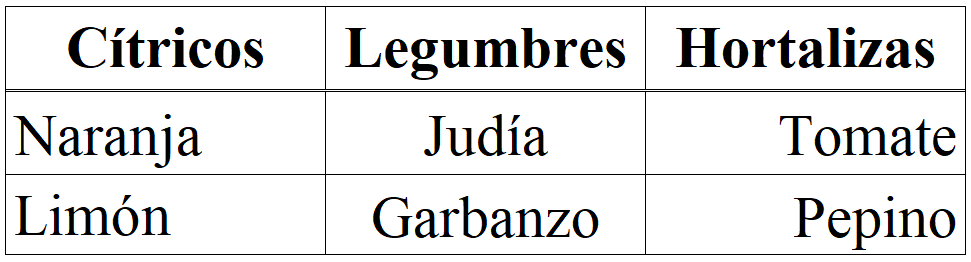
\includegraphics{alimentos}
	\end{tabular}
\end{table}

Este método es aceptable para publicaciones como TFG y Tesis. Sin embargo, no es apropiado para publicaciones especializadas (p.~ej.\ revistas y congresos) y en estos casos la editorial suele rechazar el resultado por los estándares tan exigentes empleados. El problema deriva de que las fuentes empleadas por los programas externos emplean tipografías ligeramente diferentes a las empleadas por \LaTeX.


\end{document}
